\chapter{Extremstellen/-werte}
\begin{inhalt}
  Bestimmen von
  \begin{itemize}
    \item Lokalen und globalen Extrema
    \item Sattelstellen
    \item Wendestellen
    \item Lösungen von Extremwertproblemen mit Nebenbedingungen
  \end{itemize}
\end{inhalt}

Ziemlich leicht kann man Funktionen auf sogenannte \textbf{Extremstellen} untersuchen. Das sind $x$-Werte, für die die Funktion maximal bzw. minimal ist.
\begin{bla}{Lokale Extrema}
  Es gibt zwei Arten von lokalen Extrema:
  \begin{itemize}
    \item \textbf{Lokales Minimum}: Eine Funktion $f(x)$ hat bei $x_0$ dann ein lokales Minimum, wenn in einer beliebig kleinen Umgebung von $x_0$ der Funktionswert von $x_0$ der Kleinste ist.
    \item \textbf{Lokales Maximum}: Eine Funktion $f(x)$ hat bei $x_0$ dann ein lokales Maximum, wenn in einer beliebig kleinen Umgebung von $x_0$ der Funktionswert von $x_0$ der Größte ist.
  \end{itemize}

  \begin{marginfigure}[-14em]
    \begin{tikzpicture}[
        scale=1,
        thick,
        >=stealth',
        dot/.style = {
          draw,
          fill = white,
          circle,
          inner sep = 0pt,
          minimum size = 4pt
        }
      ]
      \coordinate (O) at (0,0);

      \draw[step=1cm,gray!40] (-1.9,-0.9) grid (1.9,1.9);

      % Achsen
      \draw[->] (-2,0) -- (2,0) coordinate[label = {below:$x$}] (xmax);
      \draw[->] (0,-1) -- (0,2) coordinate[label = {right:$f(x)$}] (ymax);

      % Graph
      \draw[domain=-1.5:1.2,smooth,variable=\x,red, label={right:$f$}] plot ({\x},{-\x^3+\x^2});
      \draw (1.4,-0.2) node[red,label= {[red]below:$f$}] {};

      % y-Wert
      \draw (2/3,4/27) -- (-0.1, 4/27) {};

      % x-Wert und marker
      \draw (2/3,4/27) node[dot] {} -- (2/3,-0.1) node[label = {below:\footnotesize $\tfrac{2}{3}$}] {};
    \end{tikzpicture}
    \caption{$f(x)=-x^3+x^2$ hat bei $\frac{2}{3}$ ein lokales Maximum, aber \textbf{kein} globales!}
  \end{marginfigure}
\end{bla}

\begin{bla}{globale Extrema}
  \begin{marginfigure}
    \begin{tcolorbox}[colback=white!95!black,colframe=white!75!black,title=CAS:,arc=0mm]
      \begin{scriptsize}
        \textbf{Calculator}: \\*
        \menu{Menü > Analysis > Funktionsmaximum} \\*
          \hfill \textsc{fMax}(\( x^2 \)) \( \leadsto 0 \) \\* \ \\*
        \textbf{Graph}: \\*
        \menu{Menü > Graph anal. > Maximum > Schranken wählen}
      \end{scriptsize}
    \end{tcolorbox}
  \end{marginfigure}
  Spezielle Maxima sind die sogenannten \emph{globalen Extrema}.
  \begin{itemize}
    \item \textbf{Globales Minimum}: Hat $f(x)$ in $x_{\min}$ ein lokales Minimum und gibt es keine anderen Werte für $x$, die einen kleineren Funktionswert haben, so hat $f(x)$ in $x_0$ ein \emph{globales Minimum}.
    \item \textbf{Globales Maximum}: Hat $f(x)$ in $x_{\max}$ ein lokales Maximum und gibt es keine anderen Werte für $x$, die einen größeren Funktionswert haben, so hat $f(x)$ in $x_0$ ein \emph{globales Maximum}.
  \end{itemize}
\end{bla}

\begin{bla}{Beispiel: globale Extrema}
  $f_1(x)=x^2+1$ hat in $x_0=0$ ein globales Minimum, \\ $f_2(x)=-x^2-1$ hat in $x_0=0$ ein globales Maximum. Malt euch die Graphen auf, falls ihr sie euch nicht vorstellen könnt.
\end{bla}

\begin{bla}{Hoch- und Tiefpunkte}
  In den letzten Absätzen haben wir uns mit lokalen und globalen Extremstellen beschäftigt. Mit \emph{Extrem\textbf{stellen}} war dort stets der jeweilige $x$-Wert gemeint. Möchte man von dem Punkt sprechen, bei dem der Graph maximal beziehungsweise minimal ist, so sagt man:
  \begin{itemize}
    \item \textbf{Tiefpunkt}: Hat $f(x)$ in $x_{\min}$ ein lokales Minimum, so ist $T=(x_{\min},f(x_{\min}))$ ein \emph{Tiefpunkt} von $f$.
    \item \textbf{Hochpunkt}: Hat $f(x)$ in $x_{\max}$ ein lokales Maximum, so ist $H=(x_{\max},f(x_{\max}))$ ein \emph{Hochpunkt} von $f$.
  \end{itemize}
  \textcolor{red!75!black}{\textbf{Achtung!}} Hier besteht sehr große Verwechslungsgefahr! Achtet in Aufgabenstellungen immer sehr genau darauf, was von euch verlangt wird.
\end{bla}

\begin{bla}{Vorzeichenwechsel}
  Um im nächsten Absatz die Bedingungen für Extrema beschreiben zu können müssen wir wissen, was ein Vorzeichenwechsel ist. \\ Ein \emph{Vorzeichenwechsel} liegt an einer Stelle vor, an der der Graph der Funktion die $x$-Achse schneidet. Ein Vorzeichenwechsel kann entweder von $-$ nach $+$ oder von $+$ nach $-$ erfolgen.
\end{bla}

\begin{bla}{Bedingungen für Extrema}
  In $x_0$ kann nur eine Extremstelle vorliegen wenn $f'(x_0)=0$. Oder anders formuliert:
  \begin{itemize}
    \item \textbf{Notwendige Bedingung}: Hat $f$ in $x_0$ eine Extremstelle, so ist $f'(x_0)=0$. \\
    Hinweis: Das bedeutet, dass es $x_{\text{fake}}$ geben kann, sodass $f'(x_{fake})=0$ aber $f$ keine Extremstelle in $x_{\text{fake}}$ hat! Dies ist beispielsweise in Sattelpunkten der Fall.
  \end{itemize}
  Wir brauchen also noch eine Bedingung. Diese ist die
  \begin{itemize}
    \item \textbf{Erste hinreichende Bedingung}: Ist die notwendige Bedingung erfüllt und hat $f'$ bei $x_0$ einen Vorzeichenwechsel von $-$ nach $+$, so hat $f$ in $x_0$ ein lokales Minimum (bei einem Maximum liegt ein Vorzeichenwechsel von $+$ nach $-$ vor).
  \end{itemize}
  Oft einfacher zu vernwenden ist die
  \begin{itemize}
    \item \textbf{Zweite hinreichende Bedingung}: Ist die notwendige Bedingung erfüllt und \\ $f''(x_0)<0$, liegt also $x_0$ in einer Rechtskurve, so hat $f$ in $x_0$ ein lokales Maximum (lokales Minimum für $f''(x_0)>0$ (Linkskurve)).
  \end{itemize}
\end{bla}

\begin{bla}{Sattelstellen/-punkte}
  Ist für ein $x_0$ die notwendige Bedingung erfüllt, aber keine der beiden hinreichenden, so liegt eine Sattelstelle vor. Das bedeutet, dass $f'(x_0)=0$, aber kein Vorzeichenwechsel vorliegt. \\ Der Punkt $(x_0,f(x_0))$ ist dann ein \emph{Sattelpunkt} von $f$.
\end{bla}

\begin{marginfigure}
  \begin{tikzpicture}[
      scale=0.7,
      thick,
      >=stealth',
      dot/.style = {
        draw,
        fill = white,
        circle,
        inner sep = 0pt,
        minimum size = 4pt
      }
    ]
    \coordinate (O) at (0,0);

    \draw[step=1cm,gray!40] (-2.9,-2.9) grid (2.9,2.9);

    % Achsen
    \draw[->] (-3,0) -- (3,0) coordinate[label = {below:$x$}] (xmax);
    \draw[->] (0,-3) -- (0,3) coordinate[label = {right:$f(x)$}] (ymax);

    % Graph
    \draw[domain=-0.5:2,smooth,variable=\x,red] plot ({\x},{(\x-1)^3+1});
    \draw (2.1,2.1) node[red,label= {[red]below:$f$}] {};

    % y-Wert
    \draw (1,1) -- (-0.1, 1) node[label = {left:\footnotesize $1$}] {};

    % x-Wert und marker
    \draw (1,1) node[dot] {} -- (1,-0.1) node[label = {below:\footnotesize $1$}] {};

    % Tangente
    \draw[dashed,gray] (-2,1) -- (2.8,1);
  \end{tikzpicture}
  \caption{$f(x)={(x-1)}^3+1$ hat in $x_{\text{Sattel}}=1$ eine Sattelstelle.}
\end{marginfigure}

\begin{bla}{Wendestellen/-punkte}
  \begin{marginfigure}
    \begin{tcolorbox}[colback=white!95!black,colframe=white!75!black,title=CAS:,arc=0mm]
      \begin{scriptsize}
        \textbf{Graph}: \\*
        \menu{Menü > Graph anal. > Wendepunkt > Schranken wählen} 
      \end{scriptsize}
    \end{tcolorbox}
  \end{marginfigure}

  \begin{marginfigure}
    \begin{tikzpicture}[
        scale=0.7,
        thick,
        >=stealth',
        dot/.style = {
          draw,
          fill = white,
          circle,
          inner sep = 0pt,
          minimum size = 4pt
        }
      ]
      \coordinate (O) at (0,0);

      \draw[step=1cm,gray!40] (-4.4,-1.9) grid (4.4,1.9);

      % Achsen
      \draw[->] (-4.5,0) -- (4.5,0) coordinate[label = {below:$x$}] (xmax);
      \draw[->] (0,-2) -- (0,2) coordinate[label = {right:$f(x)$}] (ymax);

      % Graph
      \draw[domain=-4:4,smooth,variable=\x,red, label={right:$f$}] plot ({\x},{sin(deg(\x))});
      \draw (3.141592-0.5,1.3) node[red,label= {[red]below:$f$}] {};

      % Tangente
      \draw[dashed,gray] (-2,-2) -- (2,2);

      % Ursprung
      \draw (0,0) node[dot] {};
    \end{tikzpicture}
    \caption{$f(x)=\sin(x)$ hat in $x_{\text{Wende}}=0$ eine Wendestelle. Wenn man auf dem Graph von $-\infty$ nach $\infty$ fahren würde, so stünde hier das Lenkrad gerade.}
  \end{marginfigure}

  Die Stellen, an denen eine Funktion $f$ von einer Links- in eine Rechtskurve wechselt --- oder umgekehrt --- nennt man \emph{Wendestellen}. Die Bedingungen sind sehr ähnlich wie die Bedingungen für Extrema und sind graphisch leicht nachvollziehbar:
  \begin{itemize}
    \item \textbf{Notwendige Bedingung}: $f$ kann in $x_0$ nur dann eine Wendestelle haben, wenn $f''(x_0)=0$ gilt (da $f''(x_0) < 0$ für eine Rechts- und $f''(x_0) > 0$ für eine Linkskurve).
    \item \textbf{Erste hinreichende Bedingung}: Ist die notwendige Bedingung erfüllt und hat $f''$ in $x_0$ einen Vorzeichenwechsel, so hat $f$ in $x_0$ eine Wendestelle.
    \item \textbf{Zweite hinreichende Bedingung}: Ist die notwendige Bedingung erfüllt und ist $f'''(x_0)\neq 0$, so hat $f$ in $x_0$ eine Wendestelle.
  \end{itemize}
  Wie bei den Extrema definiert man für eine Wendestelle von $f$ bei $x_0$ den zugehörigen Wendepunkt $(x_0,f(x_0))$.
\end{bla}

\section{Extremwertprobleme mit Nebenbedingungen}

\begin{bla}{Beispiel: Fläche maximieren}
  \begin{marginfigure}[5em]
    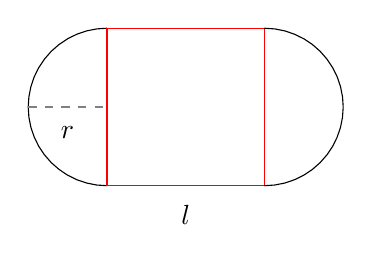
\begin{tikzpicture}
      % Laufbahn und Feld
      \draw [domain=270:90] plot ({cos(\x)}, {sin(\x)});
      \draw [domain=0:2,red] plot ({\x},{1});
      \draw [domain=0:2,red] plot ({\x},{-1});
      \draw [domain=-1:0,gray,dashed] plot ({\x},{0});
      \draw [domain=-1:1,red,variable=\y] plot ({0},{\y});
      \draw [domain=-1:1,red,variable=\y] plot ({2},{\y});
      \draw [domain=-90:90] plot ({cos(\x)+2}, {sin(\x)});

      % Beschriftung
      \draw (1,-1) node[label={below:$l$}] {};
      \draw (-0.5,0) node[label={below:$r$}] {};
    \end{tikzpicture}
    \caption{Das \textcolor{red}{Spielfeld} soll möglichst groß werden. Wie müssen $l$ und $r$ gewählt werden?}
  \end{marginfigure}
  Eine 400m-Laufbahn soll so gemacht werden, dass das rechteckige Spielfeld in der Mitte der Laufbahn möglichst groß wird. Wie sind $l$ und $r$ zu wählen, damit diese Fläche maximal wird?
\end{bla}

\begin{koch}
  \textbf{Lösungsstrategie für Extremwertprobleme mit Nebenbedingungen}:
  \begin{enumerate}
    \item Die Größe, die maximal/minimal werden soll, durch einen Term beschreiben.
    \item Bedingung in den Term einsetzen $\rightarrow$ Größe hängt nur noch von einer Variablen ab
    \item Term ableiten und Nullstellen bestimmen $\rightarrow$ Minima/Maxima der Größe
    \item Testen: Sind die Ergebnisse sinnvoll?
  \end{enumerate}
\end{koch}



\begin{bla}{Lösung des Beispiels}
  Wir lösen das Beispiel mit dem Kochrezept.
  \begin{enumerate}
    \item Die Fläche des Rechtecks wird beschrieben durch $A_{l,r}=l*2r$.
    \item Die Bedingung ist $400=2l+2\pi r$. Um die Bedingung in den obigen Term einsetzen zu können formen wir die Bedingung nach einer Variable um, beispielsweise nach $l$: $l=200-\pi r$. Wir erhalten also durch Einsetzen: $A(r)=(200-\pi r)*2r=400r-2\pi r^2$.
    \item Die Ableitung von $A(r)$ ist $A'(r)=400-4\pi r$. Als Nullstellen erhalten wir:
    \begin{equation*}
      A'(r)=0 \Leftrightarrow 400-4\pi r = 0 \Leftrightarrow 100=\pi r \Leftrightarrow r = \tfrac{100}{\pi}
    \end{equation*}
    Die beiden Kreisbögen haben also zusammen die Länge $2\pi r = 2\pi \tfrac{100}{\pi} = 200m$. Also ist $l=100m$.
    \item Wir müssen das Ergebnis nicht testen, tatsächlich ist die gerade Strecke bei einer echten $400m$-Laufbahn $100m$ lang.
  \end{enumerate}
\end{bla}
